\section{System Overview} \label{sec:overview}
\sysname enables a user $B$ to discover the \textit{message} $\msg_A$ of a user $A$ known only by its \textit{identifier} $n_A$ and the establishment of a shared cryptographic secret between these users. An identifier is a public human-readable string unique to a user, such as a phone number, an email address, or a social media handle. \sysname aims to be efficient and privacy-friendly by hiding the identifiers, messages, and relationships between users.

\subsection{Actors}
\sysname is composed of the following actors:
\begin{itemize}
    \item \textbf{Users: } A \emph{user} $A$ owns a human-readable identifier $n_A$ and a message (or payload) $\msg_A$. They wish to allow specific users to discover their message $\msg_A$ on the conditions that 1) $A$ knows the other user's identifier and 2) the other user knows $A$'s identifier $n_A$. Users wish to hide their relationships with other users from any observer.
    \item \textbf{Registration Authorities: } A \emph{registration authority} (RA) attests to the binding between users and their identifiers. A registration authority could be a social media service (e.g., Twitter) allowing the use of handles as usernames or a messaging service verifying a phone number. Identifiers always specify the registration authority that attested to them. As a result, multiple services (e.g., Signal~\cite{signal}, Telegram~\cite{telegram}, WhatsApp~\cite{whatsapp}) can all use the user's phone number as an identifier by appending their unique registrar domain, e.g., \texttt{phone\_number@domain}. A registration authority can be a single entity or a distributed set of authorities. The concrete deployment structure is decided by the respective service designers/operators. For simplicity of presentation we assume henceforth (see \Cref{sec:setup}) that a registration authority is a single entity.
    \item \textbf{Key-issuing Authorities: } The \emph{key-issuing authorities} (KAs) share a threshold key (see \Cref{sec:setup}) to issue private keys to users presenting a (blinded) identifier attested by a registration authority. \sysname assumes that at most $t$ key-issuing authorities are malicious (see \Cref{sec:assumptions}). In some cases, it is beneficial to instantiate the key-issuing authorities as a superset of a (distributed) registration authority (\Cref{sec:instantiations}).
    \item \textbf{Storage Authorities: } The \sysname storage is operated by a set of $3f+1$ independent \emph{storage authorities} out of which at most $f$ are Byzantine (see \Cref{sec:properties}). These storage authorities may coincide with the key-issuing authorities by setting $t=2f+1$; this paper however considers them separate to facilitate the integration with existing systems (see \Cref{sec:instantiations}). In the general setting, storage authorities may enforce their own access control policy and only accept write requests from users registered with registration authorities of their choice.
   \nico{Changed the threshold $t$ back to being the maximum number of malicious key-issuing authorities (rather than number of honest as I asked previously); sorry Alberto. Not sure how that affects this relation between $t$ and $f$}
\end{itemize}

\subsection{Protocol Outline} \label{sec:protocol-overview}
\sysname is divided into two phases: (i) a \emph{setup phase} where the users obtain a long-term private key over their identifier, and (ii) a \emph{discovery phase} where users use their private keys to discover the messages of other users they know by their identifier. The setup phase is executed only once (or rarely) and the discovery phase is executed every time a user wishes to make its message discoverable or discover the message of a user with a known identifier.
%
\Cref{fig:arke-overview} provides an overview of \sysname and the interactions between its actors.

\paragraph{Setup phase}
User $A$ convinces a registration authority of its ownership of a particular identifier $n_A$ and receives a signed attestation in return~(\one).
%
User $A$ then uses this attestation along with its blinded identifier $n_A$ to obtain a set of long-term private keys from the \sysname \emph{key-issuing authorities}~(\two).

\paragraph{Discovery phase}
After running the setup phase, user $A$ can make their identifier discoverable by a specific user $B$ with a known identifier. User $A$ first locally derives a cryptographic shared key with user $B$~(\three). They then write the distributed \sysname store to enable the discovery of its message by user $B$~(\four).
%
User $B$ can discover the message of user $A$ by locally deriving the shared key with user $A$~(\five) and reading the distributed \sysname store~(\six).
%
\sysname divides time in a sequence of epochs (e.g., lasting about 1 or 2 weeks). After a fixed number of epochs, the storage authorities delete the records of inactive users (see \Cref{sec:epoch-change}).


\begin{figure*}[t]
    \centering
    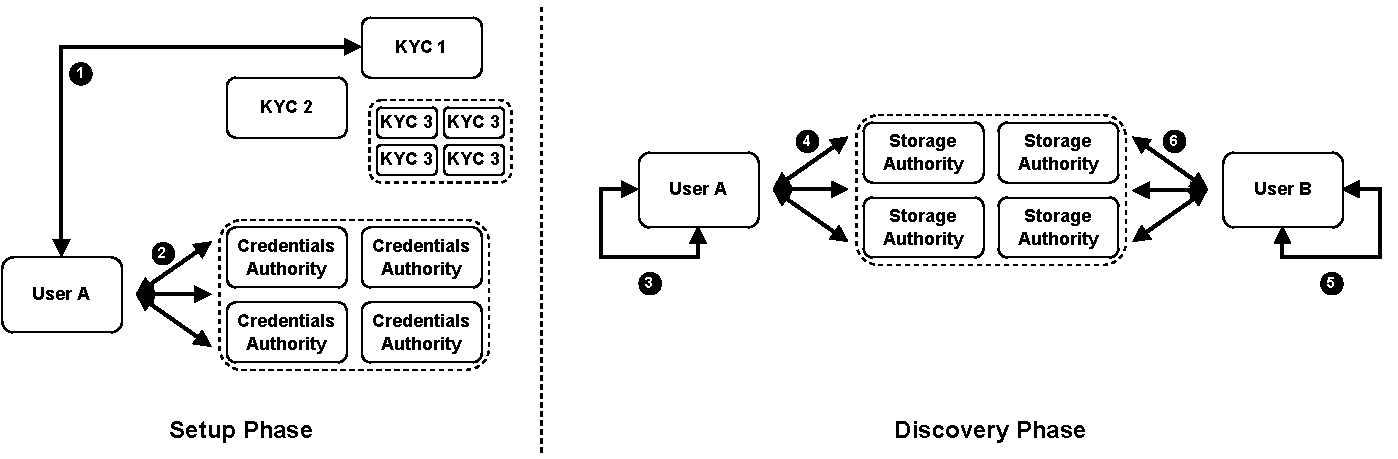
\includegraphics[width=\textwidth]{figures/arke-overview.drawio.pdf}
    \caption{
        $\sys$ overview. During the setup phase, users individually run a setup procedure with a registration authority to obtain an attestation over their identifier~(\one). They then use this attestation along with their blinded identifier to obtain a pair of long-term private keys by interacting with the key-issuing authorities~(\two). During the discovery phase, users locally derive a shared key with another user known by their identifier~(\three,\five) and use it to read and write the \sysname distributed store and discover their messages~(\four,\six).
    }
    \label{fig:arke-overview}
    \Description{}
\end{figure*}

\subsection{Design Goals} \label{sec:properties}
\sysname guarantees several system security, privacy, and performance properties.

\paragraph{System security properties}
\sysname maintains several systems security properties depending on which assumptions (\Cref{sec:assumptions}) hold. These security properties are formally defined and proved in \Cref{sec:security}.
\begin{itemize}
    \item \textbf{Validity:} A user $A$ can only update the \sysname store by updating the message associated with its identifier $n_A$.
    \item \textbf{Write consistency:} No correct storage authorities hold conflicting records.
    \item \textbf{Read consistency:} Two correct users cannot be tricked into reading different values. That is if user $B$ reads $\msg_A$ of user $A$ then user $C$ also reads $\msg_A$.
    \item \textbf{Write termination:} A correct user can eventually update the store to make its message discoverable.
    \item \textbf{Read termination:} A correct user can eventually read the store and learn the message associated with a user with a known identifier.
\end{itemize}

\paragraph{Privacy properties}
\alberto{Describe the privacy properties.}
\nico{A note on forward secrecy: as Arke is based on ID-NIKE, it does not provide forward secrecy (see Patterson and Srinivasan \cite{cryptoeprint:2007/453}). It is important that cryptographic applications such as Signal or blockchains only include "public" information in their Arke payloads to protect against future compromise of Arke private keys.}

\paragraph{Performance properties}
\sysname also guarantees the following system and performance properties. \Cref{sec:implementation_and_eval} demonstrates these properties through a thorough implementation and evaluation of \sysname.
\begin{itemize}
    \item \textbf{High-throughput:} \alberto{Show how many users we can support vs. how many users other solutions can handle (e.g. PSI-based scheme).}
    \item \textbf{Low-latency:} \alberto{Claim sub-second latency (even under load)?}
    \item \textbf{Performance under (crash-)faults:} The performance (throughput and latency) of \sysname is virtually unaffected by (crash-)faulty authorities. Note that evaluating a BFT system while experiencing Byzantine faults is an open research problem~\cite{twins}.
    \item \textbf{Linear scalability:} Authorities can take advantage of more hardware resources to linearly increase the system's throughput without impacting latency.
    \item \textbf{Bounded storage}: Storage is not growing linearly over time.
      \sysname enables authorities to periodically purge their store entries.
      This property is proven as part of \emph{consistency}.
\end{itemize}

\paragraph{Additional properties}
Furthermore, \sysname guarantees the following meta-properties:
\begin{itemize}
    \item \textbf{Censorship resistance}: Correct users can always obtain private keys from the key-issuing authorities. Furthermore correct users can write and read the \sysname store despite the presence of Byzantine authorities. This property is proved as part of \emph{write termination} and \emph{read termination}.
    \item \textbf{Authorities Non-Interactivity}: Neither the \sysname key-issuing authorities nor the storage authorities need to communicate with each other. This property allows for easier deployment and is crucial to integrate \sysname into the Sui blockchain~\cite{sui} (see \Cref{sec:instantiations}).
\end{itemize}

\subsection{Threat Model} \label{sec:assumptions}
We define the main assumptions under which \sysname guarantees the properties of \Cref{sec:properties}.

\assumption{Correct registration authorities}{\label{as:kyc}
    \sysname guarantees the security properties of \Cref{sec:properties} for identifiers issued by correct registration authorities. As mentioned in \Cref{sec:overview}, \sysname runs with a variety of registration authority. If a registration authority is malicious, it can only compromise the identifiers it attests to. That is, a corrupted registration authority \texttt{reg\_1} can compromise all interactions with identifiers of the form \texttt{user\_A@ref\_1} but the identifiers issued by other registration authority remain secure. A corrupt registration authority may attest to arbitrary bindings between users and identifiers.
}

\assumption{BFT authorities}{\label{as:bft}
    \sysname assumes a computationally bound adversary that controls the network and can corrupt at most $t$ key-issuing authorities and up to $f$ (out of $3f+1$) storage authorities in every epoch\footnote{\sysname requires quorum intersection only for the storage authorities.}. We say that authorities corrupted by the adversary are Byzantine or faulty and the rest are honest or correct. Byzantine authorities may act arbitrarily, while correct ones follow the protocol.
}

\assumption{Cryptography}{\label{as:crypto}
    The cryptographic schemes used in \sysname assume the existence of a non-degenerate and efficiently computable bilinear map $e: \GG_1 \times \GG_2 \rightarrow \GG_T$ for which the decisional bilinear Diffie-Hellman (DBDH) assumption holds. Hash functions are modeled as random oracles.
}

\assumption{Network model}{\label{as:net}
    To capture real-world networks we assume that links between users and correct authorities are reliable (the authorities do not communicate with each other). That is, all messages among the correct authorities eventually arrive. We assume a known $\Delta$ and say that execution of a protocol is eventually synchronous if there is a global stabilization time (GST) after which all messages sent among honest parties are delivered within the network delay $\Delta$ time. An execution is synchronous if GST occurs at time 0, and asynchronous if GST never occurs.
    %
    \sysname assumes an eventually synchronous network.
}

\assumption{Roughly synchronized clocks}{\label{as:clock}
    \sysname assumes that users have roughly synchronized clocks with the correct storage authorities.
    %That is, for every epoch $\Epoch$ of duration $\delta_e$, there is a period $0 < \delta \leq \delta_e$ during which the users and the correct authorities are in the same epoch $\Epoch$. Furthermore, all epochs have equal duration $\delta_e$. More formally:
    \begin{definition}[Roughly Synchronized Clocks]
      While a user is in epoch $e$, correct authorities are either in epoch $e$, $e-1$, or $e+1$. \philipp{We should probably use another notation for epochs to avoid confusion with bilinear maps.}
        Also, users remain in the same epoch each correct authority for a duration of at least $3\Delta$ (where $\Delta$ is the bound on message propagation time during periods of synchrony introduced in assumption 4).
        %Also, users and correct authority are both in epoch $e'$ for a duration of $\delta > 0$.
    \end{definition}
    % \alberto{Can we relax the assumption on "equal duration" and say that all users and correct authorities have epochs that last $\delta_e \pm \delta_e/2$?}
}
